\subsection{Importance-Informed KV Placement}
\label{sec:techb}

\subsubsection{\techBa{}}
\label{sec:techba}
% We propose the \techba{} technique to address the issue where unimportant KVs within the same chunk are also loaded and cached when retrieving important KVs. The core idea is to increase the density of important KVs within a chunk by reordering and repacking them into new chunks, thereby reducing bandwidth waste during reads. 
% This reordering and repacking process is performed periodically \wj{(e.g., 10 minutes in our settings)}, based on the average importance of each token throughout the cycle.
% The entire process is executed asynchronously, so the time spent does not impact the main I/O path.

% We introduce the \techba{} method to tackle the problem of loading and caching unimportant KVs alongside important ones within the same chunk. The essence is to enhance the concentration of important KVs in a chunk by periodically reordering and consolidating them into new chunks, which minimizes bandwidth wastage during read operations.
% This reorganization and repacking is scheduled at regular intervals (e.g., every 10 minutes in our configuration), aligned with the average importance of each token over the cycle. The entire operation is conducted asynchronously, ensuring that the time invested does not interfere with the primary I/O operations.

We present the \techba{} method to address the unnecessary loading of unimportant KVs during important KV retrieval. By periodically reorganizing and repacking important KVs into denser chunks, this approach optimizes read efficiency and reduces bandwidth waste.
Scheduled at regular intervals (e.g., every 10 minutes), this process is based on the average token importance and operates asynchronously to avoid disrupting the main I/O flow.


\begin{figure}
	\centering
	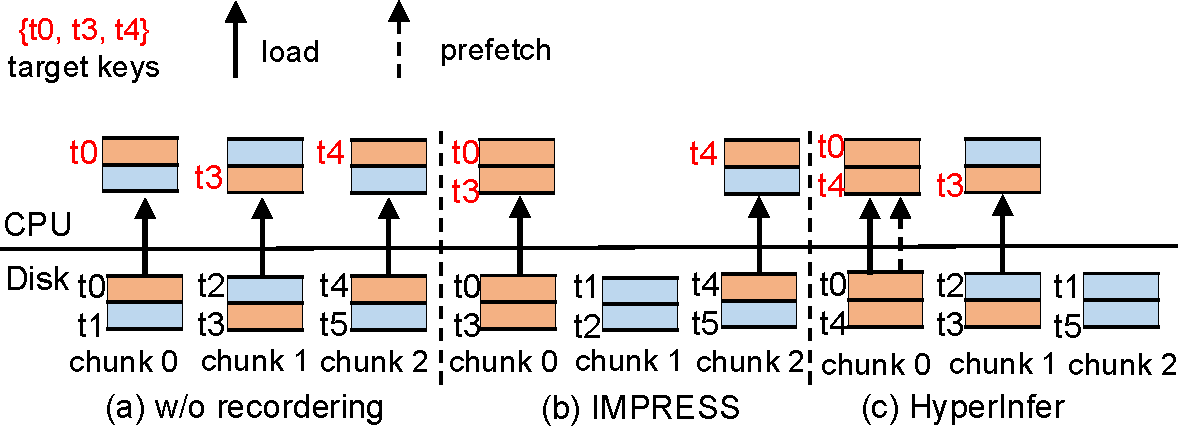
\includegraphics[width=3.4in, height=1.3in]{reorder.pdf}
%	\vspace{-0.1in}
	\caption{Comparison of the number of chunks read before and after the token sequence is reordered. The orange (blue) rectangles represent important (unimportant) keys.}
	\label{fig:reordering}
	\vspace{-0.1in}
\end{figure}

%To illustrate this process, consider an example where a prefix consists of four tokens [t0, t1, t2, t3], and the existing system stores keys for two adjacent tokens in a single chunk. Suppose each chunk contains one important key and one unimportant key.
%Figure~\ref{fig:reordering}(a) demonstrates that, without the \techba{} technique, both chunks must be loaded from disk into CPU memory to retrieve the two important keys \{t0, t3\}. This leads to unimportant keys consuming valuable read bandwidth and cache space. In contrast, with \techba{} enabled (as shown in Figure~\ref{fig:reordering}(b)), the four tokens are first reordered in a descending order of importance, and then the keys of two adjacent reordered tokens (i.e., [t0, t3] and [t1, t2]) are packed into a single chunk. This allows only one chunk to be loaded to access all two important keys, thereby reducing the amount of data read from the disk.
\fvc{
To illustrate, consider a prefix [t0, t1, t2, t3] where the existing system stores keys for two adjacent tokens in one chunk, each containing one important and one unimportant key. Without \techba{} (Figure~\ref{fig:reordering}(a)), both chunks must be loaded to retrieve the important keys \{t0, t3\}, wasting read bandwidth and cache space on unimportant keys. With \techba{} (Figure~\ref{fig:reordering}(b)), tokens are reordered by importance, and keys of adjacent reordered tokens ([t0, t3] and [t1, t2]) are packed into one chunk. This enables loading just one chunk to access all important keys, reducing disk read data.
}

%\noindent \textbf{Metadata adjustment.}
%%In LLM inference, a token's KV can only be reused when that token and all preceding tokens are identical across requests. 
%In LLMs, prefix KVs can only be reused if two prefixes share a common subsequence starting from the first token 
%(i.e., the token order must be the same).
%Therefore, existing systems typically use a radix tree~\cite{sglang-arxiv23, chunkattention-arxiv24} or its variants~\cite{ragcache-arxiv24} to record stored prefix tokens, enabling quick search for reusable stored prefix KVs when a new request arrives. 
%%However, the \techba{} could disrupt the original metadata organization, affecting the ability to check and reuse shared prefix KVs for new requests.
%However, \techba{} may destroy the radix tree structure by altering the token order, 
%causing new requests to fail in locating the correct shared prefix KVs.
%To overcome this, we limit the scope of KV reordering to the tokens within each node of the radix tree. Additionally, we introduce a mapping list within each node to assist the checking operations of new requests.
%We use an example to explain the details.
%
%\begin{figure}
%	\centering
%	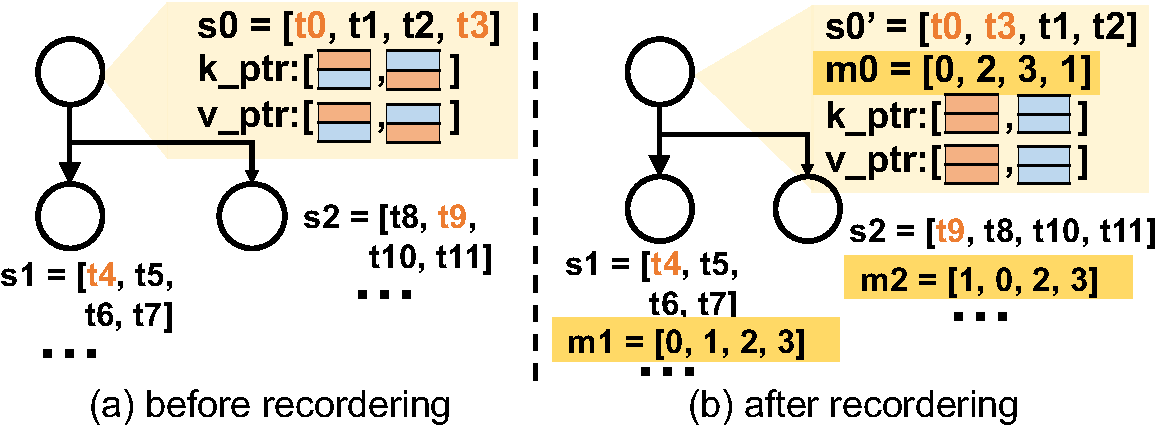
\includegraphics[width=3.3in, height=1.2in]{metaupdate.pdf}
%%	\vspace{-0.1in}
%	\caption{Comparison of meta structure before and after KV reordering. The orange (blue) rectangles represent important (unimportant) keys.}
%	\label{fig:metaupdate}
%	\vspace{-0.1in}
%\end{figure}
%
%Consider two requests that retrieve related document segments as prefixes
%through RAG. Each prefix contains eight tokens: p0=[t0, t1, t2, t3, t4, t5, t6,
%t7] for one request and p1=[t0, t1, t2, t3, t8, t9, t10, t11] for the other. t0,
%t3, t4, and t9 are important data, while the remaining tokens are unimportant.
%Before applying the \techba{} technique, the radix tree is organized as shown in
%Figure~\ref{fig:metaupdate}(a), where the common prefix subsequence s0=[t0, t1,
%t2, t3] is grouped within the same node, enabling the reuse of as many prefix
%KVs as possible. Assume the chunk size is set to 2, with each chunk containing the keys or values of two consecutive tokens.
% Each node contains a list of pointers k\_ptr (v\_ptr) to
%these key (value) chunks.
%
%After enabling \techba{}, as shown in Figure~\ref{fig:metaupdate}(b), the token sequence within each node is reordered in a descending order of importance, and the keys and values are repacked. In Node 0, for example, the token sequence becomes s0' = [t0, t3, t1, t2], with t0 and t3 now grouped within the same chunk. 
%Consequently, reordering disrupts the token sequence in the radix tree.
%We add a new mapping list to Node 0 to address this issue.
%It is denoted as m0 = [0, 2, 3, 1], allowing the original s0 sequence to be recovered using the torch index operation s0'[m0] when search reusable shared prefixes for new requests. This vectorized indexing operation is highly efficient, consuming less than 2\% of the TTFT in our experiments. 
%
%We explicitly avoid cross-node reordering, such as placing t4 and t9 into s0', for two key reasons. First, it would destroy the radix tree structure since t4 and t9 are not common tokens shared by both prefixes (i.e., p0 and p1), potentially leading to errors in retrieving reusable prefix segments for new requests. Second, it would result in unnecessary read bandwidth consumption by loading t9 when reusing the KVs of p0. The constraint against cross-node reordering prevents packing unshared tokens' KVs from different prefixes together, thereby reducing bandwidth wastage.


\subsubsection{\techBb{}}
\label{sec:techbb}
To cut down on PCIe transfers, after loading a chunk from disk into CPU
memory, only the important key and value vectors from that chunk are sent to the
GPU memory via PCIe. However, as depicted in Figure~\ref{fig:imp_token_num}, the
presence of important key or value vectors in a chunk does not align with the
chunk's access frequency. Consequently, existing systems that base their caching
decisions for GPU or CPU memory solely on recency or frequency of chunk access
may lower the GPU cache hit ratio for important key-value pairs, thus increasing
PCIe traffic.

\noindent \textbf{Score-based cache admission.}
To enhance cache efficiency, we introduce the importance-aware cache admission policy.
% \techbb{} policy.
This policy assigns a score to each chunk based on its access frequency and the
proportion of important keys or values it holds. Chunks with higher scores are
preferentially cached in GPU memory, whereas those with lower scores are stored
in CPU memory. This approach boosts the GPU cache hit ratio and minimizes data
transfers between CPU and GPU. The importance ratio is dynamically calculated as
a moving average, updating online after each chunk access.


%\begin{comment}


% For example, assume that key chunk 1 and key chunk 2 come from prefixes requested by application A and application B, respectively, and only one chunk can be stored in the GPU. Since the number of past requests from application A is 1.5 times that of application B, chunk 1 is accessed more frequently than chunk 2. However, only one key (i.e., 50\%) in chunk 1 is important, while both keys (i.e., 100\%) in chunk 2 are important. 
% As shown in Figure~\ref{fig:score_cache}(a), the existing system would place chunk 1 in the GPU and chunk 2 in the CPU because chunk 1 has a higher access frequency. When 15 new requests from application A and 10 new requests from application B arrive, this placement would result in the need to transfer 10 $\times$ 2 = 20 important keys from CPU to GPU. 
% However, considering the importance ratio, chunk 1's score would be 1.5 $\times$ 50\% = 0.75, and chunk 2's score would be 1 $\times$ 100\% = 1. Thus, chunk 2 would be placed in the GPU, as shown in Figure~\ref{fig:score_cache}(b), which would reduce the data transfer during the servicing of the 25 new requests to only 15 $\times$ 1 = 15 important keys.
%\end{comment}

For instance, suppose key chunk 1 from application A and key chunk 2 from
application B are contenders for the limited GPU memory, with application A's
request frequency being 1.5 times that of B, making chunk 1 more frequently
accessed. However, chunk 1 contains only one important key (50\%), while chunk 2
contains two important keys (100\%).
As depicted in Figure~\ref{fig:score_cache}(a), traditional systems would cache
chunk 1 in the GPU memory due to its higher access frequency, relegating chunk 2 to
the CPU. With 15 new requests from A and 10 from B, this approach would
necessitate transferring 20 important keys from CPU to GPU.
By contrast, factoring in the importance ratio, chunk 1 scores 0.75 (1.5 $\times$
50\%), and chunk 2 scores 1 (1 $\times$ 100\%). Thus, our method caches chunk 2 in
the GPU memory, as shown in Figure~\ref{fig:score_cache}(b), cutting the transfer of
important keys to just 15.

\begin{figure}
	\centering
	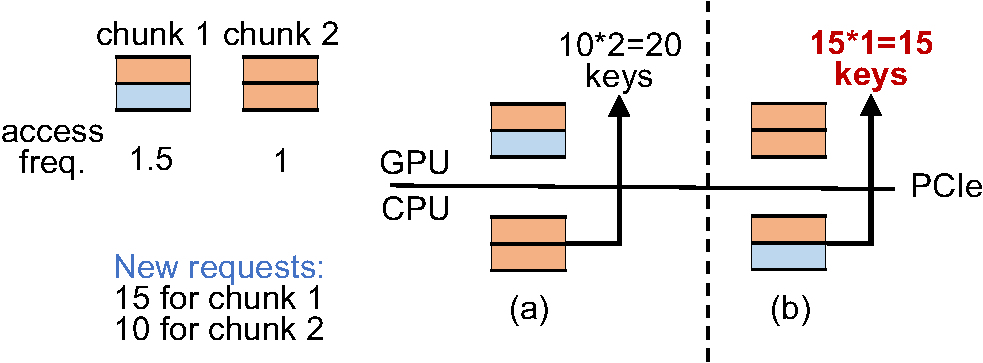
\includegraphics[width=3.3in, height=1.2in]{score_cache.pdf}
	% \vspace{-0.1in}
	\caption{Comparison of two cache replacement policies.(a) is the
	frequency-based cache replacement policy and (b) is the \techbb{} policy. The orange (blue) rectangles
	represent important (unimportant) keys. Only important keys are needed for
	new requests.}
	\label{fig:score_cache}
	\vspace{-0.1in}
\end{figure}


\begin{figure*}
	\subfigure[PIQA]{
		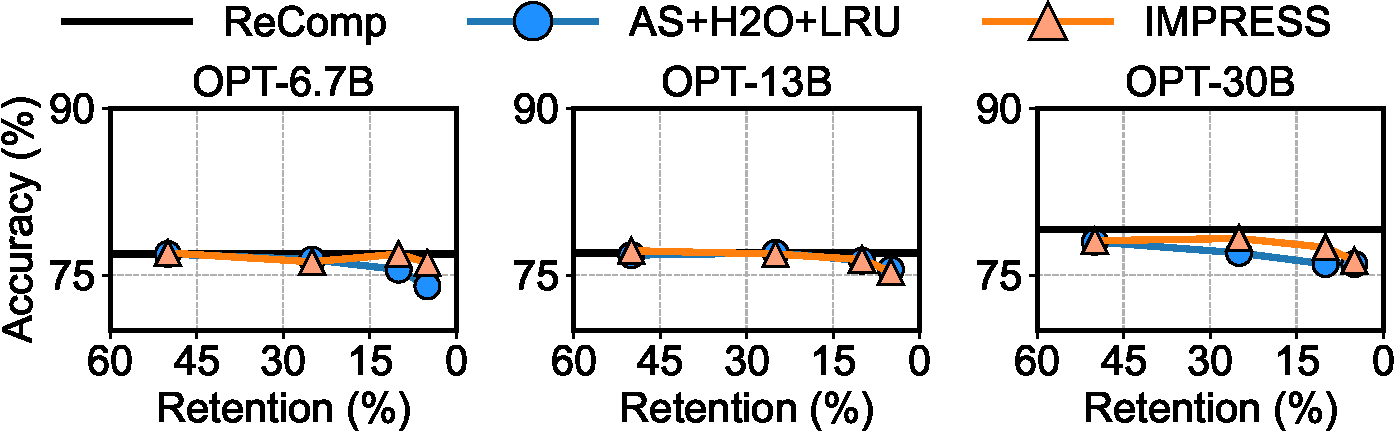
\includegraphics[width=3.3in, height=1.1in]{overall_acc1_piqa.pdf}
	}
	\hspace{0.1in}
	\subfigure[RTE]{
		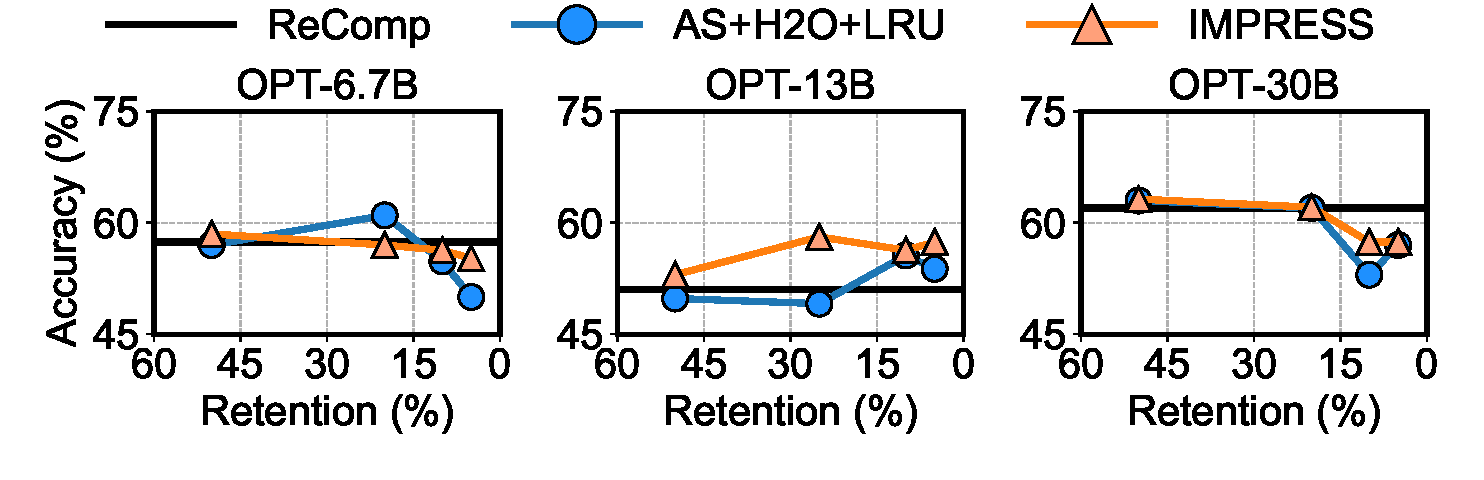
\includegraphics[width=3.3in, height=1.1in]{overall_acc1_rte.pdf}
	}
	\subfigure[COPA]{
		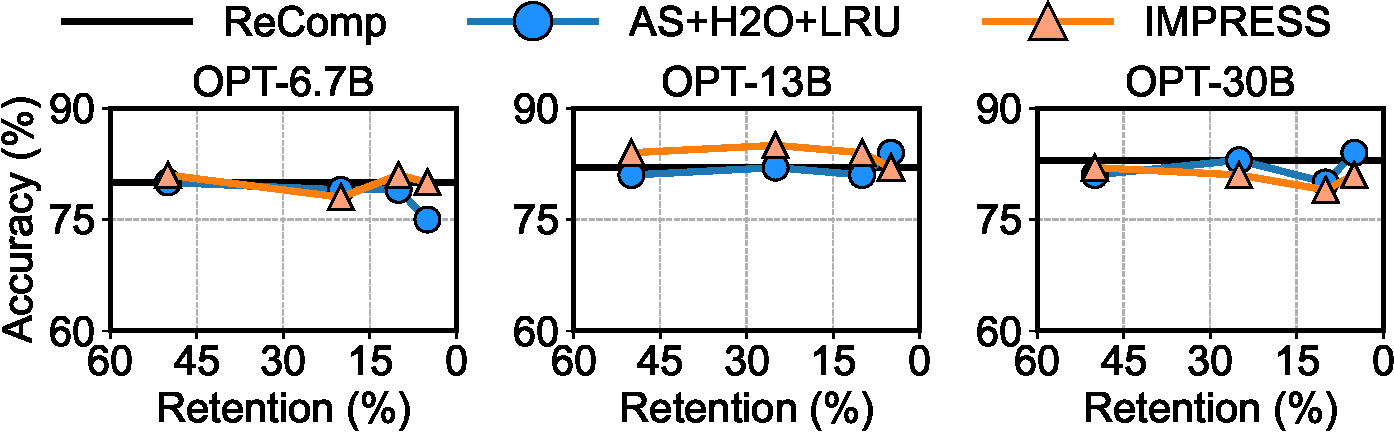
\includegraphics[width=3.3in, height=1.1in]{overall_acc1_copa.pdf}
	}
	\hspace{0.2in}
	\subfigure[OpenBookQA]{
		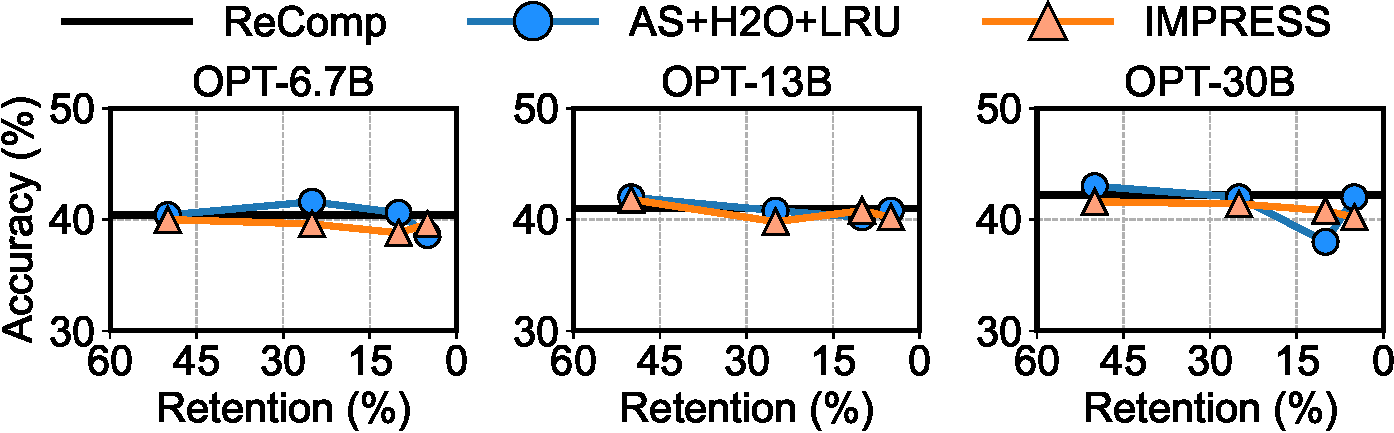
\includegraphics[width=3.3in, height=1.1in]{overall_acc1_openbookqa.pdf}
	}
	
	\vspace{-0.1in}
	\caption{
		Model generation quality of various systems across four datasets and three models.}
	\label{fig:overall_acc}
	\vspace{-0.1in}
\end{figure*}

%\noindent \textbf{Dual-cache replacement algorithm.} 
%The \pname{} system includes both GPU and CPU caches, each managed by different cache eviction strategies due to the varying granularity of data transfers from disk and CPU. Specifically, to optimize disk I/O efficiency, data is transferred from disk to CPU cache in chunks, regardless of the ratio of important KVs within each chunk. Consequently, the CPU cache eviction is only based on chunk access frequency to minimize the number of chunks loaded from the disk. 
%In contrast, when transferring data from the CPU cache to the GPU cache, only important KVs are transmitted to reduce  \ysl{the pressure on the PCIe bus}~\cite{flexgen-icml23}. Therefore, the \techbb{} method is employed in GPU cache eviction to minimize the transmission of important KVs.
%
%To achieve this, 
%we maintain two separate min-heaps in the GPU and CPU caches to assist with cache eviction. The top elements in the GPU heap are chunks with the lowest scores, while in the CPU heap, they are chunks with the lowest access frequency.
%When a new request arrives, the system first checks the radix tree-based meta data to identify reusable stored prefix KV chunks and locate whether they are located in the GPU cache, CPU cache, or disk.
%If the target chunk is in the GPU cache, after the chunk is accessed and its score is updated, it remains in the GPU cache.
%If the target chunk is in the CPU cache, its score is updated and compared with the smallest score in the GPU cache. If the target chunk's score is higher, it is swapped with the lowest-score chunk in the GPU cache; otherwise, it stays in the CPU cache.
%If the target chunk is on the disk, its access frequency is updated and compared with the lowest access frequency in the CPU cache. If the target chunk has a higher access frequency, it replaces the least-accessed chunk in the CPU; otherwise, it stays in the disk.

\noindent \textbf{Dual-cache replacement algorithm.}
% We use \techbb{} to manage both GPU and CPU caches. To achieve this, we maintain two min-heaps in CPU memory for the chunks in GPU and CPU memory to assist with cache eviction. 
% The top elements in two heaps point to the chunks with the lowest scores in the GPU and CPU caches respectively. 
% %We ensure that chunks in the GPU and CPU caches are non-redundant to maximize the amount of cached data. Additionally, 
% We ensure that all chunks' replicas are kept on disk to avoid I/O latency when evicting chunks from the CPU to disk.
We employ score-based cache replacement policy to oversee GPU and CPU caches, utilizing two min-heaps in CPU memory to manage chunks in both caches and facilitate eviction. The heaps' tops indicate the lowest-scored chunks in the GPU and CPU caches, respectively. To optimize data caching, we ensure non-redundancy between the GPU and CPU caches. Additionally, we maintain all chunk replicas on disk, thus eliminating I/O latency when chunks are evicted from CPU to disk.

Upon receiving a new request, \pname{} first identifies reusable important tokens and locates their associated chunks. If the chunk is already in the GPU cache, \pname{} utilizes the key or value vectors for inference and updates the chunk's score, retaining it in the GPU cache. If the chunk is in the CPU cache, after transferring the vectors to the GPU, \pname{} updates and compares the chunk's score with the GPU cache's lowest. If superior, it replaces the lowest-scored chunk in the GPU cache; otherwise, it stays in the CPU cache.
Should the chunk reside on disk, \pname{} loads it into CPU cache, transfers the necessary vectors to the GPU, and updates the chunk's score. This new score is then assessed against the lowest scores in both caches to decide whether the chunk should be promoted to the GPU cache, remain in the CPU cache, or stay on disk.



%\subsubsection{\techBb{}}
%当要读取的重要token的key or value vector在disk上时,\pname{} 首先会从disk加载其所在的chunk到CPU中,然后读取仅传送重要的key or value vectors 到GPU中从而减小PCIe传输量,最后决定该chunk是否被GPU或CPU缓存以备后续使用。
%However, we observed that the number of important key or value vectors in a chunk does not correlate with the chunk’s access frequency, as shown in Figure~\ref{fig:imp_token_num}. Therefore, existing systems that determine whether to cache a chunk in GPU memory or CPU memory based solely on access recency or frequency may reduce the hit ratio of important key-value pairs in the GPU cache, leading to an increase in data transferred via PCIe.
%
%To address this, we propose an importance-informed \techbb{} that further improves the GPU cache hit ratio and reduce the data transfer volume from CPU to GPU.
%The core idea is to assign a score to each chunk and use the score to determine whether it should be cached. 
%This score is defined as the cumulative number of important vectors accessed within each chunk.
%as its access frequency multiplied by the ratio of important keys or values it contains. 
%The chunks with higher scores are prioritized for caching in GPU memory, while those with lower scores are placed in CPU memory. 
%The score is updated after each chunk access.
% The ratio of important keys or values is computed as the moving average between two consecutive accesses and updated online after each chunk access.
%
%假设有三个chunk的访问频率分别是8, 10, 7;其中重要的token的数量分别是3, 1, 2。假设GPU和CPU都只能存储1个chunk,新的一些请求分别要访问8、10、7次三个chunk以获取其中重要的token用于推理。
%传统方法使用LFU缓存时会根据chunk访问频率从高到底放置如图x。那么传统方法一共需要经过PCIe传输8*3 + 7*2 = 38个vector。
%使用\techbb{}后,由于chunk1的score大于chunk2的score,因此放置如图x;那么一共需要经过PCIe传输10*1 + 7*2 = 24个vector。
